%% Copyright 2007-2020 Elsevier Ltd
%% 
%% This file is part of the 'Elsarticle Bundle'.
%% ---------------------------------------------
%% 
%% It may be distributed under the conditions of the LaTeX Project Public
%% License, either version 1.2 of this license or (at your option) any
%% later version.  The latest version of this license is in
%%    http://www.latex-project.org/lppl.txt
%% and version 1.2 or later is part of all distributions of LaTeX
%% version 1999/12/01 or later.
%% 
%% The list of all files belonging to the 'Elsarticle Bundle' is
%% given in the file `manifest.txt'.
%% 
%% Template article for Elsevier's document class `elsarticle'
%% with harvard style bibliographic references

\documentclass[review,12pt,authoryear]{elsarticle}

%% Use the option review to obtain double line spacing
%% \documentclass[authoryear,preprint,review,12pt]{elsarticle}

%% Use the options 1p,twocolumn; 3p; 3p,twocolumn; 5p; or 5p,twocolumn
%% for a journal layout:
%% \documentclass[final,1p,times,authoryear]{elsarticle}
%% \documentclass[final,1p,times,twocolumn,authoryear]{elsarticle}
%% \documentclass[final,3p,times,authoryear]{elsarticle}
%% \documentclass[final,3p,times,twocolumn,authoryear]{elsarticle}
%% \documentclass[final,5p,times,authoryear]{elsarticle}
%% \documentclass[final,5p,times,twocolumn,authoryear]{elsarticle}

%% For including figures, graphicx.sty has been loaded in
%% elsarticle.cls. If you prefer to use the old commands
%% please give \usepackage{epsfig}

%% The amssymb package provides various useful mathematical symbols
\usepackage{amssymb}
%% The amsthm package provides extended theorem environments
%% \usepackage{amsthm}

%% The lineno packages adds line numbers. Start line numbering with
%% \begin{linenumbers}, end it with \end{linenumbers}. Or switch it on
%% for the whole article with \linenumbers.
\usepackage{lineno}

% for adjusting table width automatically
\usepackage{adjustbox}
\usepackage{tabulary, ragged2e}
\usepackage{booktabs}

\journal{Geography and Sustainability}
%1.Full Length Article A full-length article should be a substantial and in-depth research study regarding a particular state of issue through several techniques or approaches. 
% The main text should be approximately 6,000 words in length, but it should not exceed 8,000 words (excluding abstract, references, tables, figures, and appendices).
%A maximum of 250 words abstract and up to 10 displayed items (figures and tables) is allowed. A full-length article should include an Introduction,
%Materials and methods, Results, Discussion, Conclusions, and References, which can be accompanied by Supplementary material.


\begin{document}
\begin{linenumbers}
\begin{frontmatter}
%% Title, authors and addresses
%% use the tnoteref command within \title for footnotes;
%% use the tnotetext command for theassociated footnote;
%% use the fnref command within \author or \affiliation for footnotes;
%% use the fntext command for theassociated footnote;
%% use the corref command within \author for corresponding author footnotes;
%% use the cortext command for theassociated footnote;
%% use the ead command for the email address,
%% and the form \ead[url] for the home page:
%% \title{Title\tnoteref{label1}}
%% \tnotetext[label1]{}
%% \author{Name\corref{cor1}\fnref{label2}}
%% \ead{email address}
%% \ead[url]{home page}
%% \fntext[label2]{}
%% \cortext[cor1]{}
%% \affiliation{organization={},
%%            addressline={}, 
%%            city={},
%%            postcode={}, 
%%            state={},
%%            country={}}
%% \fntext[label3]{}
\title{An exploratory analysis of the influence of resource use on the yield verse quality trade-off in Australian vineyards}
%% use optional labels to link authors explicitly to addresses:
%% \author[label1,label2]{}
%% \affiliation[label1]{organization={},
%%             addressline={},
%%             city={},
%%             postcode={},
%%             state={},
%%             country={}}
%%
%% \affiliation[label2]{organization={},
%%             addressline={},
%%             city={},
%%             postcode={},
%%             state={},
%%             country={}}
\affiliation[label1]{organization={QUT},
  addressline={},
  city={},
  postcode={},
  state={QLD},
  country={}}
\affiliation[label2]{organization={AWRI},
  addressline={},
  city={},
  postcode={},
  state={SA},
  country={}}
\affiliation[label3]{organization={Food Agility CRC},
  addressline={},
  city={},
  postcode={},
  state={Vic},
  country={}}
\author[label1,label2,label3]{Bryce Polley}
\date{20/06/2023}
\begin{abstract}
%% Text of abstract
\end{abstract}
%%Graphical abstract`
\begin{graphicalabstract}
  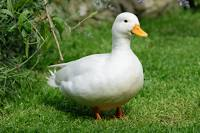
\includegraphics{graphical_abstract.jpeg}
\end{graphicalabstract}'

\begin{keyword}
%% keywords here, in the form: keyword \sep keyword
Keyword one \sep{} keyword two
%% PACS codes here, in the form: \PACS code \sep code
\PACS{} 0000 \sep{} 1111
%% MSC codes here, in the form: \MSC code \sep code
%% or \MSC[2008] code \sep code (2000 is the default)
\MSC{} 0000 \sep{} 1111
\end{keyword}
%%Research highlights
\begin{highlights}
  \item Research highlight 1
  \item Research highlight 2
\end{highlights}
\end{frontmatter}

%%%%%%%%%%%%%%%%%%%%%%%%%%%%%%%%%%%%%%%%%%
%%                main text             %%
%%%%%%%%%%%%%%%%%%%%%%%%%%%%%%%%%%%%%%%%%%

\section{Introduction}
The global focus on sustainability in agronomic industries has changed the way in which these enterprises do business. When strategies for a sustainable winegrowing industry are assessed, there is a trade-off between balancing the amount of resources invested and the resultant yield verses quality produced. This dilemma exists across agriculture through shared fundamental considerations such as water use and nitrogen levels \citep{hemmingCherryTomatoProduction2020,kawasakiQualityMattersMore2016, zhuEffectsNitrogenLevel2017}. Quality in viticulture (the cultivation of grapes for wine production) is driven through its integration within the wine industry; with a wine's potential quality being initially defined through the chemical makeup of the grapes used in its production. The consideration of sustainability within viticulture is further complicated by environmental and socio-demographic pressures. In the Australian context, these include: biosecurity, climate and international market demands.
\newline
In this analysis we observe relationships between yield and quality through the use of linear models. Although an extensive amount of research into a variety of factors' effect on grape quality and yield exists; due to the lack of long-term and in-depth data, individual effects are often studied in isolation \citep{abbalDecisionSupportSystem2016}. The lack of consolidated datasets also restricts the ability to gain statistical insights at large scales and across multiple regions \citep{keithjonesAustralianWineIndustry2002,knightFirmResourcesDevelopment2019}. The dataset used for this analysis includes data collected for the past 10 years from a multitude of vineyards located over a diverse range of Australian winegrowing regions.
\newline
We aim to use this broad dataset to confirm the existence of a yield verse quality trade off within Australian winegrowing; one not prior confirmed explicitly across such extensive diversities.
% you require a reference here
In achieving this, the context of how resource-use relates to yield and quality will also be described.
% Describing baselines is more important - it needs to be emphasised more so than something that is known but not shown. This is the heart of what your are doing sell it more.
We link these relations to the potential for improvement through decision-making processes, whilst highlighting that the way moving forward will require the optimisation of these processes. The practical addition of these aims is a baseline for comparison - given a vineyard within Australia, one could extrapolate their comparative efficiency with regard to the tradeoff between invested resources, yield and quality.
\section{Methods}
We created four linear models to explore relationships between resource-use and vineyard outputs (see Table\ref{tab:tab1}). The data was sourced from Sustainable Winegrowing Australia and Wine Australia. Variables used included: yield, average sale price, region, water use, emissions, area harvested and year. After fitting to the data, each model was validated using k-fold cross validation.
\begin{table}[]
      \caption{Summary of models; their predictors, covariates and variable interactions.}\label{tab:tab1}
        \resizebox{\textwidth}{!}{\begin{tabular}{@{}ccccc@{}}
          \toprule
          & \textbf{Response} & \textbf{Predictors} & \textbf{Covariates} & \textbf{Interactions} \\ \midrule
          \textbf{Model 1} & Yield & \begin{tabular}[c]{@{}c@{}}Water Used\\ Scope 1 Emissions\end{tabular} & \begin{tabular}[c]{@{}c@{}}Area Harvested\\ Year\\ GI Region\end{tabular} & N/A \\
          \multicolumn{1}{l}{} & \multicolumn{1}{l}{} & \multicolumn{1}{l}{} & \multicolumn{1}{l}{} & \multicolumn{1}{l}{} \\
          \textbf{Model 2} & ${ \textrm{Yield}}\over{ \textrm{Area Harvested}}$ & \begin{tabular}[c]{@{}c@{}}Water Used\\ Scope 1 Emissions\end{tabular} & \begin{tabular}[c]{@{}c@{}}Area Harvested\\ Year\\ GI Region\end{tabular} & \begin{tabular}[c]{@{}c@{}}Area Harvested * Scope 1 Emissions\\ Area Harvested * Water Use\\ Year * Region\end{tabular} \\
          \multicolumn{1}{l}{} & \multicolumn{1}{l}{} & \multicolumn{1}{l}{} & \multicolumn{1}{l}{} & \multicolumn{1}{l}{} \\
          \textbf{Model 3} & {$\textrm{Yield} {\times} \textrm{Average Sale Price}$} & \begin{tabular}[c]{@{}c@{}}Water Used\\ Scope 1 Emissions\end{tabular} & \begin{tabular}[c]{@{}c@{}}Area Harvested\\ Year\\ GI Region\end{tabular} & N/A \\
          \multicolumn{1}{l}{} & \multicolumn{1}{l}{} & \multicolumn{1}{l}{} & \multicolumn{1}{l}{} & \multicolumn{1}{l}{} \\
          \textbf{Model 4} & ${\textrm{Yield} \times \textrm{Average Sale Price}}\over{\textrm{Area Harvested}}$ & \begin{tabular}[c]{@{}c@{}}Water Used\\ Scope 1 Emissions\end{tabular} & \begin{tabular}[c]{@{}c@{}}Area Harvested\\ Year\\ GI Region\end{tabular} & \begin{tabular}[c]{@{}c@{}}Area Harvested * Scope 1 Emissions\\ Area Harvested * Water Use\\ Year * Region\end{tabular}
          \end{tabular}}
\end{table}
\subsection{Analysis}
Before models were fit to the data, Pearson Correlation Coefficients were used to look at the existence of linear relationships between predictor variables. These relationships were summarised in correlation matrices to compare the level of interaction present between predictor variables. The relationships between the predictors and response variables were then modelled using General Linear Models. Both the Pearson Correlation Coefficients and General Linear Models were created using the R statistical programming language \citep{rcoreteamLanguageEnvironmentStatistical2021}. General Linear Models were chosen as they offer the ability to produce statistical models that are explicit in the relationships between predictors and response variables.
%reference?
General Linear Models also allow the exploration of interactions between predictors and present easily comparable differences in the influence and magnitude of relationships.
% reference?
 A variety of alternate methods were also explored, including: Splines, hierarchical regression, General Additive Models, and Generalised Linear Models. These alternative approaches were not used as final models due to offering no further insights or improvements in accuracy.
\newline
The response variables of the models were yield and quality. Yield was defined as the total tonnes of grapes harvested. For the purpose of this study, quality was defined by the financial value of winegrape crops' average sale price per tonne. The definition of quality was an important consideration, as quality can be defined in a variety of ways, for example analysing grapes': aroma, chemical composition and color.
% References to were this was done.
Using sale price as a defining trait of quality was due to the market value of winegrapes being reliant on grape quality and because Wine Australia explicitly defines grape quality through the use of discrete price brackets in their annual reports
% We need a reference to where they did this
% Did they do this more prolifically at some point as well?
; the generalisation made to reflect quality through using average price assumed a due diligence of those who purchased the grapes \citep{yeggeInfluenceSensoryNonsensory2001}.  Both response variables were examined as totals and as scales of area harvested. Values were compared in this manner to observe how economies of scale affect the use of resources.
%
%
%
\subsection{Significant Tests}
%This briefly needs to be described. You use the results of significance tests in the results section and talk about variables significance but do not describe it in the methods.
%
% F-tests
%
% T-tests
%
%
\subsection{Data}
Data used in this analysis was sampled by Sustainable Winegrowing Australia and Wine Australia. Sustainable Winegrowing Australia is Australia's national wine industry sustainability program, which aims to facilitate grape-growers and winemakers in demonstrating and improving their sustainability \citep{swaSustainableWingrowingAustralia2022}. Wine Australia is an Australian Government statutory authority governed by the Wine Australia Act 2013 \citep{WineAustraliaAct2019}.
\newline
Data sampled by Wine Australia was collected via phone surveys and included: summary statistics such as yield and average price of sale per tonne; these values were summarised by region and grape varietal. Data recorded by Sustainable Winegrowing Australia was entered manually by winegrowers using a web based interface with some fields being optional, variables included: region, harvest year, yield, area harvested, water used and fuel used (diesel, petrol, biodiesel and LPG). To enable direct comparisons between fuels, they were converted to tonnes of Carbon Dioxide equivalent.
% They were converted to emissions that was expressed in TCO2E - not into the units!
\newline
The inclusion of Wine Australia data was due to average sale price being an optional field in Sustainable Winegrowing Australia's dataset. 
Regional average prices from Wine Australia were filled into values that were missing from the Sustainable Winegrowing Australia data; the common practice of purchasing grapes at regional prices was an important consideration in this decision.
%{It would be lovely to have a reference for this but it is currently only anacdotal.}
Two subsets of data were then created for the analysis. The first subset contained all vineyards and was used for Models 1 and 3. The second subset contained vineyards which either recorded a value for average price of sale per tonne through Sustainable Winegrowing Australia, or were within a region with an average price of sale recorded by Wine Australia; this subset was used for Models 2 and 4. These subsets meant that the data would be limited to samples which had recorded values for the response variables (see Table\ref{tab:tab1}), where every sample had a recorded value for yield but not average price of sale per tonne.
\newline
The first subset of data was used for Model 1 and Model 2 (see Table\ref{tab:tab1}). This subset contained 5298 samples spanning the period from 2012 to 2022, covering 55 GI Regions and 1261 separate vineyards.
\newline
The second subset of data, was limited to vineyards that recorded a value for their average sale price of grapes per tonne. This subset was used for Model 3 and Model 4 (see Table\ref{tab:tab1}); and contained 2878 samples spanning the period from 2015 to 2022, covering 51 GI Regions and 944 separate vineyards. 1842 of the values for average price of sale per tonne were extracted from Wine Australia surveys with the remaining 1036 being from Sustainable Winegrowing Australia's dataset.
\newline
Additional variables were considered for analysis but were excluded due to being either underreported or had insignificant contributions to model accuracies. Variables explored but not used due to low reporting values included: fertiliser, and scope 2 emissions. Variables considered but ultimately removed due to a lack of significant contributions to models, included: the use of renewable energy, contractor use, and pressures such as frost, fire and disease.
\newline
Data preprocessing was conducted prior to analysis using the Python programming language \citep{g.vanrossumPythonTutorialTechnical1995}. Preprocessing included logarithmic transformations, centring and scaling by standard deviation. Variables such as scope 1, which required prior calculations were also computed using Python.
% Two values for average sale price were removed from the dataset, due to a recording of \$1. 
% \citep{wineaustraliaNationalVintageReport2019,wineaustraliaNationalVintageReport2020,wineaustraliaNationalVintageReport2021,wineaustraliaNationalVintageReport2022,winemakersfederationofaustraliaNationalVintageReport2012,winemakersfederationofaustraliaNationalVintageReport2013,winemakersfederationofaustraliaNationalVintageReport2014,winemakersfederationofaustraliaNationalVintageReport2015,winemakersfederationofaustraliaNationalVintageReport2016,winemakersfederationofaustraliaNationalVintageReport2017,winemakersfederationofaustraliaNationalVintageReport2018}.
\subsection{Total Emissions}
The equation given from the Australian National Greenhouse Accounts Factors, shown as
\newline
\begin{equation}
\label{(1)}
    tCO_{2}e={{Q \times EC \times EF1 + EF3}\over{1000}},
\end{equation}
\newline
was used to convert the quantity of fuel in litres, $Q$, using a prescribed Energy Content, $EC$, and emission factors of scope one, $EF1$, and scope three, $EF3$, to tonnes of Carbon Dioxide equivalent, $tCO2e$ \citep{departmentofclimatechangeenergytheenvironmentandwaterAustralianNationalGreenhouse2022}. Emissions were calculated for total diesel, petrol, bio-diesel and LPG used. 
%\newline
% What the hell is the below paragraph and why is it here?
%The variables were reviewed for correlations by using a Pearson's Correlation Coefficient (see Tables 1, 2 and 3). This was undertaken for data on the original scale (see Table 1) and for data as a logarithmic transform (see Table 2). All P-values were found to be significant (< 2.200E-16), except the non-transformed values for water used (see Table 3). The logarithmic transforms performed the best due to a skew likely caused by a greater number of smaller vineyards within the dataset (see Table 4).
\subsection{Region}
Differences in vineyard locations were captured through the use of Geographical Indicator Regions (GI Regions). Each GI Region has its own unique mixture of climatic and geophysical properties that describes a unique winegrowing region within Australia; these regions were predefined by Wine Australia \citep{hallidayAustralianWineEncyclopedia2009,oliverReviewSoilPhysical2013,soarClimateDriversRed2008}. Both Wine Australia and Sustainable Winegrowing Australia used the same GI Region format to describe location.
\newline
The site of a vineyard predetermines several physical parameters such as climate, geology and soil; making location a widely considered key determinant of grape yield and quality \citep{abbalDecisionSupportSystem2016,agostaRegionalClimateVariability2012,fragaMultivariateClusteringViticultural2017}. The climatic properties of each GI Region were summarised by using predefined classifications as per the \citet{sustainablewinegrowingaustraliaSustainableWinegrowingAustralia2021} user manual. The user manual describes climates by rainfall and temperature, creating supersets of Regions of similar climatic properties. The climatic groups were used to illustrate similarities and differences occurring in areas larger than GI Regions.
\subsection{Model Validation}
Models were validated using K-fold cross validation calculated through the R Caret Package \citep{kuhnBuildingPredictiveModels2008}. K-fold cross validation works by removing a subset of data from the sample used to train models and then predicts those variables to determine how sensitive the model is to changes in the sample data. For this analysis each model was validated using 10 folds, repeated 100 times.
% A reference for this is absolutely needed.
\section{Results}
\subsection{Exploratory Analysis}\label{sec:exp_anal}
Linear relationships between variables were explored using Pearson Correlation Coefficients. Values for these coefficients reflect the linear relation between two variables, on a scale between -1 and 1; the magnitude and sign of a coefficient indicates the strength of the relation, and whether the relation is positive or negative respectively. This was undertaken for data on the original scale (see Table ??) and for data as a logarithmic transform (see Table ??). The logarithmic transformed data showed the strongest correlations, likely due to a skew caused by a greater number of smaller vineyards within the dataset (see Table ??). Transforming data prior to calculating the coefficients changes several things: The logarithmic transform of the data alters the interpretation of the coefficients to percentage change - a coefficient will be indicative of the change in percentage of one variable compared to the other; scaling by standard deviation also changes this interpretation to be a percentage of that variables standard deviation. Scaling by standard deviation also makes the Pearson Correlation Coefficient equal to the covariance of the two variables. With all this in mind, when considering the logarithmically transformed variables, a coefficient of 1 would indicate that: given the change of one variable by one percentage of its standard deviation, the other variable would change by one percent of its own standard deviation. The importance of this is the dimensionless nature of these relationships and that it can be translated directly to any vineyard's case that has a well known distribution.
\newline
To determine if a coefficient was indicative of a strong relationship, confidence intervals were used. P-values reflected the significance of a given correlation coefficient when considering its relation to sample size via its incorporation as an element of standard error. Strong relationships were found to be present as all P-values, except for the non-transformed values for water used, were considered significant (P $<$ 2.200E-16).
\subsection{General Linear Models}
General Linear Models were used to describe how response variables related to predictors' values. Log transformed variables were used as inputs to these models as they resulted in higher $R^2$ values and described the relationships proportionally; reflecting coefficient values as percentages of a variable's standard deviation.
\begin{table}[]
  \caption{Summary of models; their performance, F-statistics and Residual error.}\label{tab:modelsummary}
      \resizebox{\textwidth}{!}{
        \begin{tabular}{@{}cccccccc@{}}
          \toprule
           & $\mathbf{R^2}$ & $\mathbf{R^2}$ & \textbf{F-Statistic} & \textbf{P-Value} & \textbf{\begin{tabular}[c]{@{}c@{}}Residual\\ Standard Error\end{tabular}} & \textbf{\begin{tabular}[c]{@{}c@{}}Residual Sum\\ of Squares\end{tabular}} & \textbf{\begin{tabular}[c]{@{}c@{}}Residual Mean\\ of Squares\end{tabular}} \\ \midrule
          \textbf{\begin{tabular}[c]{@{}c@{}}Model 1\\ Yield\end{tabular}} & 9.072E-01 & 9.061E-01 & 7.753E+02 & 2.200e-16 & 3.065E-01 & 4.913E+02 & 1.000E-01 \\
          \multicolumn{1}{l}{} & \multicolumn{1}{l}{} & \multicolumn{1}{l}{} & \multicolumn{1}{l}{} & \multicolumn{1}{l}{} & \multicolumn{1}{l}{} & \multicolumn{1}{l}{} & \multicolumn{1}{l}{} \\
          \textbf{\begin{tabular}[c]{@{}c@{}}Model 2\\ Yield/Area\end{tabular}} & 7.951E-01 & 7.770E-01 & 4.403E+01 & 2.200e-16 & 4.722E-01 & 1.085E+03 & 2.200E-01 \\
          \multicolumn{1}{l}{} & \multicolumn{1}{l}{} & \multicolumn{1}{l}{} & \multicolumn{1}{l}{} & \multicolumn{1}{l}{} & \multicolumn{1}{l}{} & \multicolumn{1}{l}{} & \multicolumn{1}{l}{} \\
          \textbf{\begin{tabular}[c]{@{}c@{}}Model 3\\ Value\end{tabular}} & 9.753E-01 & 9.748E-01 & 1.885E+03 & 2.200e-16 & 1.589E-01 & 7.111E+01 & 3.000E-02 \\
          \multicolumn{1}{l}{} & \multicolumn{1}{l}{} & \multicolumn{1}{l}{} & \multicolumn{1}{l}{} & \multicolumn{1}{l}{} & \multicolumn{1}{l}{} & \multicolumn{1}{l}{} & \multicolumn{1}{l}{} \\
          \textbf{\begin{tabular}[c]{@{}c@{}}Model 4\\ Value / Area\end{tabular}} & 9.669E-01 & 9.638E-01 & 3.095E+02 & 2.200e-16 & 1.904E-01 & 9.528E+01 & 4.000E-02 \\ \bottomrule
          \end{tabular}
        }
\end{table}
Each model showed a strong relationship between the predictors and the response (see Table~\ref{tab:modelsummary}). Model accuracy was measured in $R^2$, as this allowed an easy comparison between their performances and their validation.
\subsubsection{F-tests}
To determine if predictors significantly related to a Model's response variable, F-tests were conducted. Aside from 3 variables, all F-tests across each model indicated a significant contribution at 95\% confidence. The three exceptions were: scope 1 emissions in Model 3 (P=2.221E-01) and Model 4 (P=3.621E-01), and Model 2's interaction between area harvested and water used (P=2.192E-01).
\newline
Scope 1 emissions was included in all models to directly compare the response variables as ratios of vineyard size to raw values. Even though not significant within models 3 and 4, when using the Pearson Correlation Coefficients scope 1 emissions was strongly correlated to every Model's response variable; this was especially so for Model 1 and 4 (Yield and average price per tonne as a ratio to area harvested, respectively).
\subsubsection{T-tests}
T-tests were used to determine if predictors significantly contributed to their models when accounting for other variables; this allowed a more granular examination of interactions and factors within categorical variables, showing which specific years and areas contributed significantly and which did not (the appendix contains a comprehensive list of these values). 
\newline
For Models 1 (yield) and 3 (value) year played a pivotal role, with only one year in each model not being significant (2021/2022 and 2016/2017 respectively). Both Model 1 and 3 showed a majority of regions were significant with 32 of 54 regions being significant in Model 1, and 42 of 50 regions being significant in Model 3 with 95\% confidence.
\newline
The number of combinations of year and region meant that Models 2 and 4 had many tests (424 and 243 respectively). Model 2 found 62.56\% of these combinations were indicative of a significant contribution to the model at 95\% significance. Model 4 was found to have 88.07\% of its year/region combinations indicating a significant contribution. A likely reason for some combinations not being significant was a lack of samples in that particular region/year being present; with region sample sizes ranging from 1 to 1006.
\newline
With regard to continuous variables, Model 1 and 2 showed water use, scope 1 emissions and area harvested were significant at 95\% confidence when accounting for other variables. T-tests for Model 3 showed all continuous variables except scope 1 emissions were significant. Model 4 showed scope 1 emissions and water use to only be significant when considered as an interaction with area harvested but not when considered on their own.
\subsubsection{Model Coefficients}
%
% What are you trying to say here?
% Coefficients are important as they describe the direct relationship between a variable and its response. They indicate whether it is a positive, or negative relationship and the magnitude of this relationship.
The coefficients of each model describe the relationship of a predictor variable to its response when considering all other variables. Due to the transformations of the data, coefficients are individually interpreted in the same manner as the prior regression values were (see Section \ref{sec:exp_anal}); unlike the regression values,  coefficient ranges are not limited between -1 and 1, as each variable needs to be considered together.
%The dimensionless nature of these variables each coefficient refers to its own variable's distribution's standard deviations.
\newline
We look at the coefficients of categorical and continuous variables separately. This is primarily done as the categorical variables have many coefficients, one for each category, whilst continuous variables have only one. The coefficient for categorical variables is summarised in Figure\ref{fig:violin}; illustrating the difference in the range as well as affect region and year could have on each of the models. Comparatively, the continuous variables coefficients are summarised in Table \ref{tab:contvar}.
In terms of magnitude, GI region has the highest possible absolute value for each model. An important consideration is that region and year are binary, such that they are only equal to zero or the coefficient (as they will present as a value of 1 which will be multiplied by the coefficient); this means that, although region may have a strong relationship, it can be overshadowed by an extreme value of one of the continuous variables. The most notable difference between the continuous variables coefficients is the change from positive to negative values. This change occurs between the Models for Yield (Model 1 and 2) and the Models for value (Models 3 and 4); where all but the coefficient for area harvested had the opposite sign. These models also differ in an order of magnitude when looking at resource use, with the coefficients for yield being smaller than those for value. 
%
% The resource input is different by an order of magnitude between value and yield
%
% Area has the strongest nfluence
%
% The models as a ratio of area show opposite trends - this could be indicative that smaller vineyards tend twoards more valuable crops and larger to crops of greater yield. 
%
\begin{figure}
  \caption{Violin plots of GI Region and Year coefficients for each model.}\label{fig:violin}
  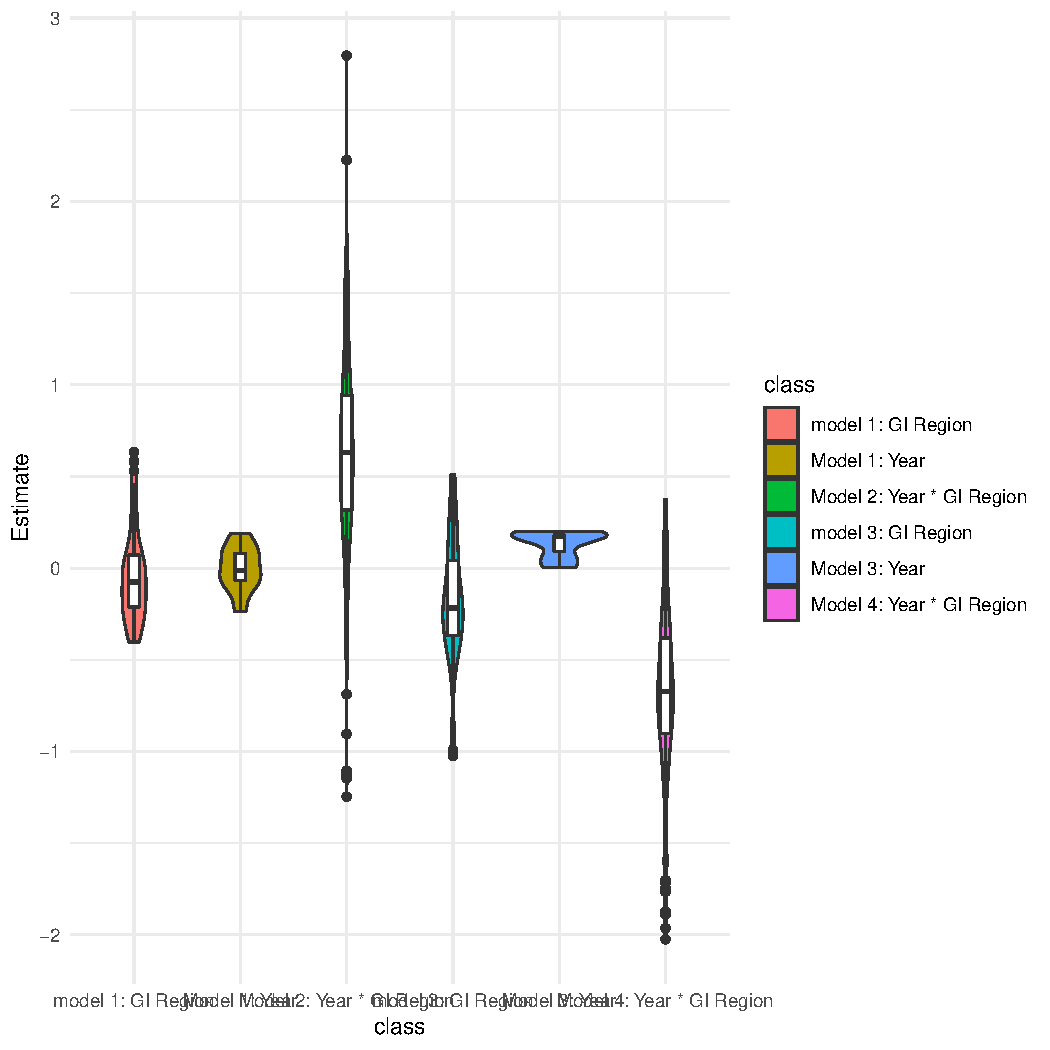
\includegraphics{violinplot.pdf}
  \end{figure}
%
\begin{table}[]
  \caption{Summary of each Models coefficients for continuous variables}\label{tab:contvar}
      \resizebox{\textwidth}{!}{
        \begin{tabular}{@{}cllllll@{}}
          \toprule
           & \textbf{Intercept} & \multicolumn{1}{c}{\textbf{\begin{tabular}[c]{@{}c@{}}Area\\ Harvested\end{tabular}}} & \multicolumn{1}{c}{\textbf{\begin{tabular}[c]{@{}c@{}}Water\\ Used\end{tabular}}} & \multicolumn{1}{c}{\textbf{\begin{tabular}[c]{@{}c@{}}Scope 1\\ Emissions\end{tabular}}} & \multicolumn{1}{c}{\textbf{\begin{tabular}[c]{@{}c@{}}Area\\ Harvested\\ $\ast$\\ Scope 1\\ Emissions\end{tabular}}} & \multicolumn{1}{c}{\textbf{\begin{tabular}[c]{@{}c@{}}Area\\ Harvested\\ $\ast$\\ Water\\ Used\end{tabular}}} \\ \midrule
          \textbf{Model 1} & -3.318E-02 & 7.418E-01 & 8.660E-02 & 6.731E-02 &  &  \\
          \textbf{Model 2} & -6.516E-01 & 5.774E-01 & 1.079E-02 & 8.498E-02 & -4.971E-02 & -5.346E-02 \\
          \textbf{Model 3} & 1.808E-02 & 9.713E-01 & -2.310E-02 & -6.992E-03 &  &  \\
          \textbf{Model 4} & 6.702E-01 & -7.354E-01 & -6.732E-03 & -5.645E-03 & 2.726E-02 & 7.515E-02 \\ \bottomrule
          \end{tabular}}
\end{table}
\subsubsection{Model Comparisons: Yield Verse Value}
%
\begin{figure}\label{fig:yield_vs_value}
  \resizebox{\textwidth}{!}{
  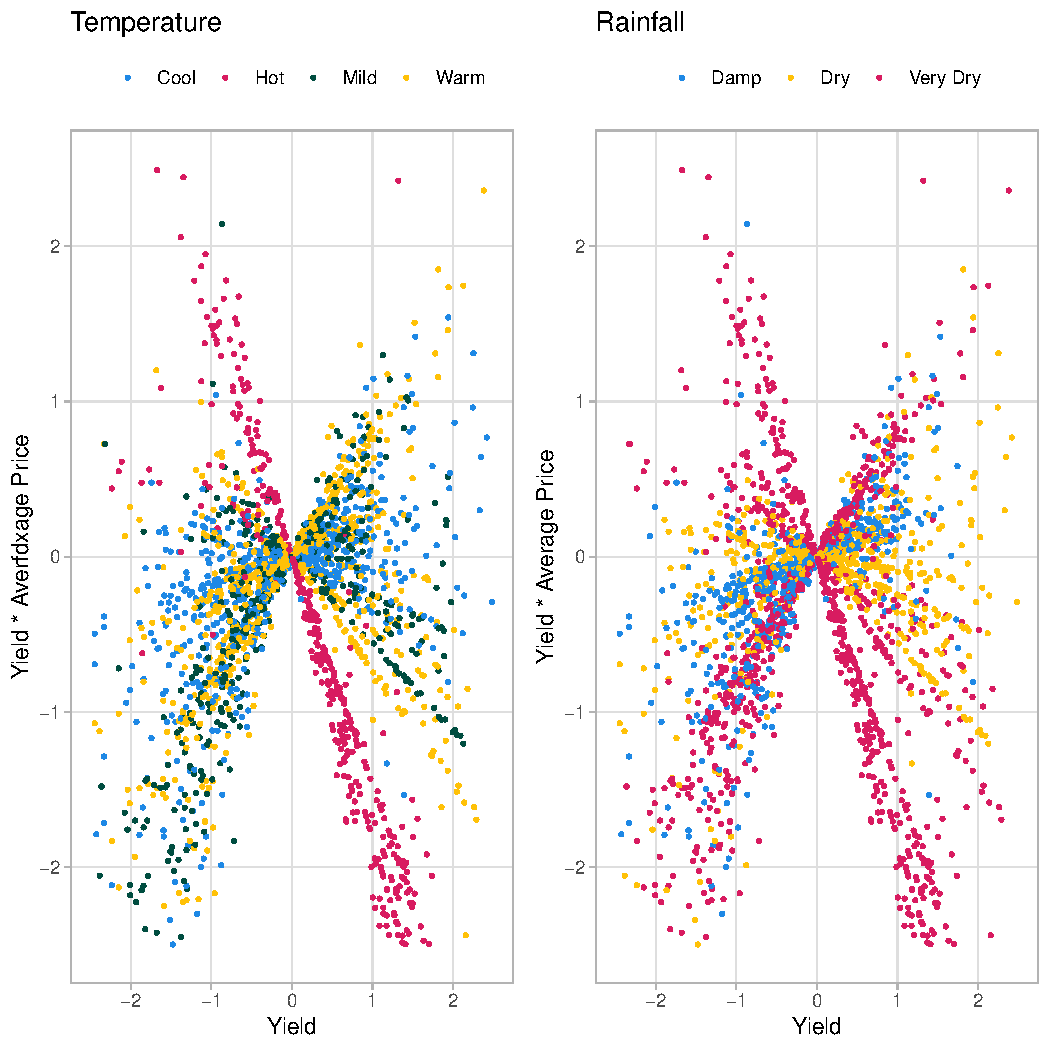
\includegraphics{yield_verse_value.pdf}}
  \caption{Scatter plot of vineyard yield against the product of yield and average price per tonne. The axes are in standard deviations with points coloured by climate.}
\end{figure}
%
\begin{figure}\label{fig:yield_vs_value_area}
  \resizebox{\textwidth}{!}{
  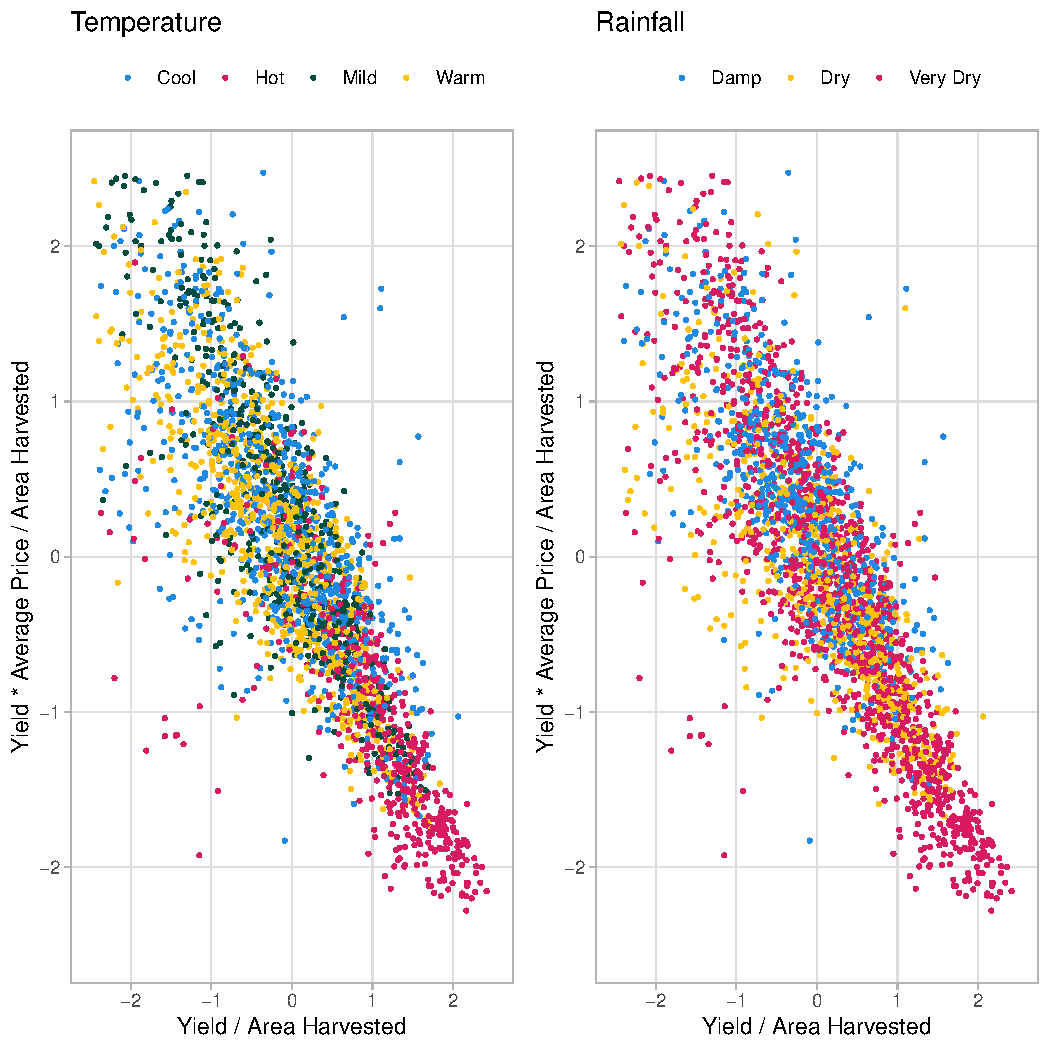
\includegraphics{yield_verse_value_by_area.pdf}}
    \caption{Scatter plot of vineyard yield against the product of yield and average price per tonne as ratios to area harvested. The axes are in standard deviations with points coloured by climate.}
\end{figure}
% wHY ARE WE COMPARING MODELS?
% We compare models to see which predictors contributed relatively to each of the models.
%
%Models were compared using $R^2$ values. The comparison of models performance showed that the average price per tonne of grapes describes a great deal of the relationship between predictor and response when comparing Model 2 to Model 4 
% Graph of productivity verse value.
%(see Table \ref*{tab:modelperformance}). 
% This is important but you do not illustrate why
%
% This section needs to be heavily revised. Why are there tails on the distributions? What does a heavy tail indicate?
% What does it look like with respect to disaster events?
% split the discussion sections out of the results!! Even the questions I am asking are answered in the discussion, however they need to be highlighted as aspects of the models here beforehand.
 Reviewing the data to uncover reasons for this included the use of binary variables such as the utilisation of renewable energy, contractors, and the occurrence of disease, fire and frost; however none of these variables were able to explain why some vineyards produced less, or why other vineyards sold at higher prices than predicted. A wide variety of these influences were likely already explained within the use of year and GI Region, or the interaction of both variables. The change between some regions was dramatic, with particularly warmer and drier regions producing much higher volumes of grapes at lower prices (See Figures 5 and 6). The use of other variables and methods, specifically splines, were able to create a more normally distributed set of residuals but at a drastically reduced accuracy when comparing R2 and RSE. The introduction of known average prices per tonne also helped increase R2 values a small amount; it is important to not that it is common practice for wineries to purchase grapes at a regional average rate, likely resulting in much less variance within a region.

different strategies are likely employed between different regions, where some regions target the mass production of cheaper grapes over quality. This is most notable when grouping regions by climate, especially when considering GI Regions in the 'Hot Very Dry' climate (see Figure 7). The effect of climate in the models was not more significant than the more granular use of GI regions. The interaction between year and GI Region likely accounted for localised events such as bushfires, which would be impactful, but only at a local level in both time and space.

\subsection{Model Validation}
To validate the performance of these models k-fold cross validation was used. This was done using 10 folds, $k=10$, repeated 100 times. The models performed similarly to their original counter parts (see Table \ref*{tab:kfold}).
\begin{table}[]
  \label{tab:kfold}
  \caption{Model validation using k-fold cross validation, for 10 folds repeated 100 times.}
  \begin{tabular}{cccc}
          & RMSE      & R2        & MAE       \\
  Model 1 & 3.087E-01 & 9.045E-01 & 2.165E-01 \\
  Model 2 & 5.104E-01 & 7.409E-01 & 3.493E-01 \\
  Model 3 & 1.652E-01 & 9.723E-01 & 1.008E-01 \\
  Model 4 & 2.235E-01 & 9.500E-01 & 1.279E-01
  \end{tabular}
  \end{table}
\section{Discussion}
% We want to compare how much influence each variable has on the model!
% This is prior to postulating about the why these variables matter, or have so much influence.
% 
% A table will help to compare the continuous variables, the others are done in the violin plot.
%
% What is this below paragraph?
%The correlation between average sales price and yield was a negative trend (see table 2); the contributing factors to yield and average sales price was ???. Correlation values showed that water and emissions increased with yield but decreased with average sale price (see Table 4).
%
In alternative attempts at models it was found that without the incorporation of GI Region or year the predictions greatly under performed. The possible reason behind this effect was that different strategies are likely employed between different regions, where some regions target the mass production of cheaper grapes over quality. % ALSO THAT CATASTROPHES HAPPEN EVEN ON SMALL SCALES THis needs to be tied up better.
%
\subsection{Limitations}
Limitations included overestimating yield for models 1 and 2, (see Figures 1 and 2) and underestimating crop value in models 3 and 4 (see Figures 3 and 4).
% this needs serious revision.
This study investigated the general relationships between input resources of a vineyard, including fuel and water, and the outputs including yield and value. Some regions appeared to produce many low quality grapes at scale compared to attempting to produce fewer higher quality grapes. This behaviour can be observed when reviewing Wine Australia's annual reports, where it is apparent that warm inland regions such as the Riverland are known to only produce large amounts of lower graded grapes \cite{wineaustraliaNationalVintageReport2022,winemakersfederationofaustraliaNationalVintageReport2017}. Comparatively, regions such as Tasmania only produce A grade grapes but in much smaller quantities than the Riverland. Knowing that the difference in pricing per tonne can exceed a magnitude of 10 between grades E and A, the operations in regions that target different grades would have varied priorities. However, some regions such as the Yarra Valley produce a Variety of different grades of grapes, from C to A, highlighting that vineyard priorities, although may be somewhat present within regional classifications, are not necessarily aligned within a given region. 

The opportunity to target different grades of grapes may not always be available, with some regions being more renowned than others, and likely to be sought after regardless \citep{hallidayAustralianWineEncyclopedia2009}. The Barossa is an example of this, known for its quality could also lend itself to a bias in purchasers not considering other regions that may be capable of similar quality. This effect could stifle the potential for market opportunities within these lesser known regions. A further possibility is that there may be regional upper limits with the relationship between resource input and the value gained becoming no longer proportional due to diminishing returns. Climate was considered to be a large determinant of the ability to grow a larger quantity of grapes, as well as a determinant in grape quality \citep{agostaRegionalClimateVariability2012}; however there were vineyards in similar regions that were able to produce exceptionally better results than others (See Figure 7).

The issue of model 1 and 2 over predicting yield, may have been due to preventative measures brought on by regional pressures such as fire, frost and disease. Where, more resources were required to prevent these issues from spreading within a region, thus disproportionately effecting some vineyards compared to others locally. This type of maintenance is not well captured especially when considering that some regions, those in warmer areas are not as prone to disease as cooler climates and could potentially have lower operating costs per hectare. This could create a discrepancy in vineyards that utilise preventative measures in wetter regions, as opposed to those who do not, and thus expend less fuel and energy but risk disease. When reviewing the differences between regions it is important to consider that vineyards in Hot Very Dry areas can be hundreds of times the size of those in other regions. It is interesting that while area, although significantly correlated to the ratio of yield to area, was still lower than water and about the same as emissions. This points to economies of scale playing a role but still being only one consideration alongside the potential resources that can be used. The negative trend between size and average sales price could also be a side effect of mass supply verse demand, especially when looking at the level of difference in production of some vineyards (see Table 4). The relationships between yield, value and area are not simply about efficiently producing the most grapes; sales price and by association grape quality, are integral to the profitability, and this is strongly linked to resource-use and thus the longevity and sustainability of a vineyard. 

Literature shows that there are many on-the-ground decisions that influence both quality and yield. Where these decisions are governed by complex physical and social forces such as international market demands, disease pressures and natural disasters \citep{abadCoverCropsViticulture2021,cortezUsingDataMining2009,hallWithinseasonTemporalVariation2011,i.goodwinManagingSoilWater2009,kasimatiPredictingGrapeSugar2022,oliverReviewSoilPhysical2013,srivastavaNondestructiveSensingMethods2018}. Many of these occurrences being highlighted throughout the past decades vintage reports \citep{wineaustraliaNationalVintageReport2019,wineaustraliaNationalVintageReport2021,wineaustraliaNationalVintageReport2022,winemakersfederationofaustraliaNationalVintageReport2013,winemakersfederationofaustraliaNationalVintageReport2014,winemakersfederationofaustraliaNationalVintageReport2015,winemakersfederationofaustraliaNationalVintageReport2016,winemakersfederationofaustraliaNationalVintageReport2017,winemakersfederationofaustraliaNationalVintageReport2018}. %This definitely needs to be broken up, what were these occurences, which year was significant for what?
It is also important to consider that these reports show that the warm inland regions have seen a decline in profit during this period, as they were often compared to other regions that focused more on quality than quantity. This is an important consideration, as the size of some of these vineyards when considering their ratio of value to area would only require a marginal increase to out compete other regions. There are also differences when comparing winegrowers to other agricultural industries as they are vertically integrated within the wine industry, tying them to secondary and tertiary industries, such as wine production, packaging, transport and sales. This results in unique issues and considerations for each vineyard, where these on-the-ground decisions may be influenced by other wine industry's choices, such as the use of sustainable practices in vineyards as a requirement for sale in overseas markets; notably these interactions are further complicated by some winegrowers being totally integrated into wine companies, while others are not (Knight et al., 2019). Incorporating such decisions into the model could help describe the contributing factors to regional differences beyond resource consumption and regional differences. 

Having more data for each region would also be an improvement, allowing greater comparison between regions. More variables may also help to discern vineyards that can produce larger volumes of grapes at higher prices. The use of semi transparent tools such as random forests and decision trees alongside more variables and data may help to uncover the reasons for values that were under or over estimated. These differences could be caused by the use of alternative sustainable practices in the field. While there is evidence to suggest that environmentally sustainable practices can reduce costs, increase efficiency, whilst improving the quality of grapes, more research is needed to link these benefits across different regions and climates \citep{baianoOverviewSustainabilityWine2021,marianiSustainableWinegrowingCurrent2015,montalvo-falconSustainabilityResearchWine2023}.

% This belongs in the discussion
The relationship between scope one emissions and the response variables that included average sales price

It is possible that the relationships between scope one emissions and the response variables were closely tied to a vineyards area. This possibility could be explained through the emissions 

Noting that irrigation systems use fuel
and that the application of water was a significant variable in each model
scope one emissions' lack of significance and contribution given its F-statistics (See Tables 7 and 8),
 indicated that it is possible other vineyard activities requiring fuel are not as determining factors for a vineyards grape quality.

\bibliography{references}
\bibliographystyle{elsarticle-harv}

%% The Appendices part is started with the command \appendix;
%% appendix sections are then done as normal sections
 \appendix


 \begin{table}[]
  \centering
  \caption{Summary of models, their predictors, covariates and variable interactions.}
  \label{tab:tab2}
  \begin{tabulary}{\textwidth}{CCCCCCCC}
  Variable                             & Yield      & Area       & Water Used & Scope One Emissions & $\textrm{Yield}\over\textrm{Area}$ & Average Price Per Tonne & ${\textrm{Average Price per tonne}\over\textrm{Area}}$ \\
  Yield                                & 1.000E+00  & 7.440E-01  & -4.309E-03 & 7.290E-01           & 3.500E-01            & -2.262E-01              & -1.644E-01                           \\
  Area                                 & 7.440E-01  & 1.000E+00  & -5.331E-03 & 8.921E-01           & 7.854E-02            & -1.178E-01              & -2.042E-01                           \\
  Water Used                           & -4.309E-03 & -5.331E-03 & 1.000E+00  & -1.929E-03          & -5.600E-03           & -3.562E-02              & -2.669E-02                           \\
  Scope One Emissions                  & 7.290E-01  & 8.921E-01  & -1.929E-03 & 1.000E+00           & 9.357E-02            & -9.422E-02              & -1.933E-01                           \\
  $\textrm{Yield}\over\textrm{Area}$                 & 3.500E-01  & 7.854E-02  & -5.600E-03 & 9.357E-02           & 1.000E+00            & -4.849E-01              & -1.698E-01                           \\
  Average Price Per Tonne              & -2.262E-01 & -1.178E-01 & -3.562E-02 & -9.422E-02          & -4.849E-01           & 1.000E+00               & 4.732E-01                            \\
  ${\textrm{Average Price per tonne}\over\textrm{Area}}$ & -1.644E-01 & -2.042E-01 & -2.669E-02 & -1.933E-01          & -1.698E-01           & 4.732E-01               & 1.000E+00                           
  \end{tabulary}
  \end{table}

  \begin{table}[]
    \caption{Pearson correlation coefficients for each logarithmically transformed variable.}
    \label{tab:tab3}
    \begin{tabular}{clllllll}
    Variable                                           & \multicolumn{1}{c}{Yield} & \multicolumn{1}{c}{Area} & \multicolumn{1}{c}{Water Used} & \multicolumn{1}{c}{Scope One Emissions} & \multicolumn{1}{c}{$\textrm{Yield}\over\textrm{Area}$} & \multicolumn{1}{c}{Average Price Per Tonne} & \multicolumn{1}{c}{${\textrm{Average Price per tonne}\over\textrm{Area}}$} \\
    Yield                                              & 1.000E+00                 & 8.822E-01                & 8.245E-01                      & 7.617E-01                               & 9.353E-01                                          & -4.591E-01                                  & -8.918E-01                                                             \\
    Area                                               & 8.822E-01                 & 1.000E+00                & 7.750E-01                      & 8.311E-01                               & 6.742E-01                                          & -1.911E-01                                  & -8.474E-01                                                             \\
    Water Used                                         & 8.245E-01                 & 7.750E-01                & 1.000E+00                      & 6.668E-01                               & 7.292E-01                                          & -4.881E-01                                  & -8.300E-01                                                             \\
    Scope One Emissions                                & 7.617E-01                 & 8.311E-01                & 6.668E-01                      & 1.000E+00                               & 6.086E-01                                          & -1.559E-01                                  & -7.063E-01                                                             \\
    $\textrm{Yield}\over\textrm{Area}$                     & 9.353E-01                 & 6.742E-01                & 7.292E-01                      & 6.086E-01                               & 1.000E+00                                          & -5.625E-01                                  & -8.076E-01                                                             \\
    Average Price Per Tonne                            & -4.591E-01                & -1.911E-01               & -4.881E-01                     & -1.559E-01                              & -5.625E-01                                         & 1.000E+00                                   & 6.592E-01                                                              \\
    ${\textrm{Average Price per tonne}\over\textrm{Area}}$ & -8.918E-01                & -8.474E-01               & -8.300E-01                     & -7.063E-01                              & -8.076E-01                                         & 6.592E-01                                   & 1.000E+00                                                             
    \end{tabular}
    \end{table}

    \begin{table}[]
      \caption{P-values for the non-transformed water used variable's Pearson correlation coefficients.}
    \label{tab:tab4}
      \begin{tabular}{cl}
      Variable                                           & Water Used \\
      Yield                                              & 7.538E-01  \\
      Area                                               & 6.981E-01  \\
      Scope One Emissions                                & 8.883E-01  \\
      $\textrm{Yield}\over\textrm{Area}$                     & 6.836E-01  \\
      Average Price Per Tonne                            & 5.600E-02  \\
      ${\textrm{Average Price per tonne}\over\textrm{Area}}$ & 1.522E-01 
      \end{tabular}
      \end{table}

    \begin{table}[]
      \caption{Summary statistics for each variable on the original scale..}
      \label{tab:tab5}
      \begin{tabular}{clllllll}
      Variable &
        \multicolumn{1}{c}{Yield} &
        \multicolumn{1}{c}{Area} &
        \multicolumn{1}{c}{Water Used} &
        \multicolumn{1}{c}{Scope One Emissions} &
        \multicolumn{1}{c}{$\textrm{Yield}\over\textrm{Area}$} &
        \multicolumn{1}{c}{Average Price Per Tonne} &
        \multicolumn{1}{c}{${\textrm{Average Price per tonne}\over\textrm{Area}}$} \\
      Yield                                              & 1.000E+00  & 8.822E-01  & 8.245E-01  & 7.617E-01  & 9.353E-01  & -4.591E-01 & -8.918E-01 \\
      Area                                               & 8.822E-01  & 1.000E+00  & 7.750E-01  & 8.311E-01  & 6.742E-01  & -1.911E-01 & -8.474E-01 \\
      Water Used                                         & 8.245E-01  & 7.750E-01  & 1.000E+00  & 6.668E-01  & 7.292E-01  & -4.881E-01 & -8.300E-01 \\
      Scope One Emissions                                & 7.617E-01  & 8.311E-01  & 6.668E-01  & 1.000E+00  & 6.086E-01  & -1.559E-01 & -7.063E-01 \\
      $\textrm{Yield}\over\textrm{Area}$                     & 9.353E-01  & 6.742E-01  & 7.292E-01  & 6.086E-01  & 1.000E+00  & -5.625E-01 & -8.076E-01 \\
      Average Price Per Tonne                            & -4.591E-01 & -1.911E-01 & -4.881E-01 & -1.559E-01 & -5.625E-01 & 1.000E+00  & 6.592E-01  \\
      ${\textrm{Average Price per tonne}\over\textrm{Area}}$ & -8.918E-01 & -8.474E-01 & -8.300E-01 & -7.063E-01 & -8.076E-01 & 6.592E-01  & 1.000E+00 
      \end{tabular}
      \end{table}
% should these tables all go into the appendix solely or should they be summarised as well?
%\begin{table}[]
%  \begin{tabular}{lllll}
%                    & Coef      & Std. Error & t-value   & Pr(\textgreater{}|t|) \\
%  Area Harvested    & 7.418E-01 & 1.003E-02  & 7.390E+01 & 2.000E-16             \\
%  Water Used        & 8.660E-02 & 8.885E-03  & 9.747E+00 & 2.000E-16             \\
%  Scope 1 Emissions & 6.731E-02 & 8.013E-03  & 8.400E+00 & 2.000E-16            
%  \end{tabular}
%  \end{table}
%
\begin{table}[]
  \label{tab:tab6}
  \caption{Model 1 ANOVA summarising variable significance at the .5 level.}
  \begin{tabular}{llllll}
  Variable       & Df & Sum Sq    & Mean Sq   & F Value   & Pr(\textgreater{}F) \\
  Year                & 9  & 7.060E+01 & 7.800E+00 & 8.353E+01 & \textless 2.20E-16 \\
  GI Region           & 54 & 1.507E+03 & 2.790E+01 & 2.972E+02 & \textless 2.20E-16 \\
  Area Harvested      & 1  & 3.211E+03 & 3.211E+03 & 3.419E+04 & \textless 2.20E-16 \\
  Water Used          & 1  & 1.040E+01 & 1.040E+01 & 1.103E+02 & \textless 2.20E-16 \\
  Scope One Emissions & 1  & 6.600E+00 & 6.600E+00 & 7.056E+01 & \textless 2.20E-16
  \end{tabular}
\end{table}
\begin{table}[]
  \label{tab:tab7}
  \caption{Model 2 ANOVA summarising variable significance at the .5 level.}
  \begin{tabular}{llllll}
  Variable                    & Df  & Sum Sq    & Mean Sq   & F Value   & Pr(\textgreater{}F)    \\
  Area Harvested              & 1   & 2.407E+03 & 2.407E+03 & 1.080E+04 & \textless 2.20E-16 *** \\
  Scope One Emissions         & 1   & 3.989E+01 & 3.989E+01 & 1.789E+02 & \textless 2.20E-16 *** \\
  Water Used                  & 1   & 5.500E+02 & 5.500E+02 & 2.467E+03 & \textless 2.20E-16 *** \\
  Area Harvested*Scope One Emissions & 1 & 6.921E+01 & 6.921E+01 & 3.104E+02 & \textless 2.20E-16 *** \\
  Area Harvested * Water Used & 1   & 1.040E+00 & 1.040E+00 & 4.686E+00 & 3.045E-02 **           \\
  Year * GI Region            & 424 & 1.144E+03 & 2.700E+00 & 1.210E+01 & \textless 2.20E-16 ***
  \end{tabular}
\end{table}
%
\begin{table}[]
  \caption{Model 3 ANOVA summarising variable significance at the .5 level.}
  \label{tab:tab8}
  \begin{tabular}{llllll}
  Variable            & Df & Sum Sq    & Mean Sq   & F Value   & Pr(\textgreater{}F)    \\
  Year                & 6  & 1.324E+01 & 2.210E+00 & 8.748E+01 & \textless 2.20E-16 *** \\
  GI Region           & 50 & 6.498E+02 & 1.300E+01 & 5.151E+02 & \textless 2.20E-16 *** \\
  Area Harvested      & 1  & 2.142E+03 & 2.142E+03 & 8.491E+04 & \textless 2.20E-16 *** \\
  Water Used          & 1  & 3.200E-01 & 3.200E-01 & 1.259E+01 & 3.947E-04 **           \\
  Scope One Emissions & 1  & 4.000E-02 & 4.000E-02 & 1.492E+00 & 2.221E-01             
  \end{tabular}
\end{table}

\begin{table}[]
\label{tab:tab9}
\caption{Model 4 ANOVA summarising variable significance at the .5 level.}
\begin{tabular}{llllll}
Variable            & Df  & Sum Sq    & Mean Sq   & F Value   & Pr(\textgreater{}F)    \\
Area Harvested      & 1   & 2.066E+03 & 2.066E+03 & 5.700E+04 & \textless 2.20E-16 *** \\
Scope One Emissions & 1   & 6.000E-02 & 6.000E-02 & 1.569E+00 & 2.105E-01              \\
Water Used          & 1   & 2.014E+02 & 2.014E+02 & 5.557E+03 & \textless 2.20E-16 *** \\
Area Harvested*Scope One Emissions & 1 & 5.246E+01 & 5.246E+01 & 1.448E+03 & \textless 2.20E-16 *** \\
Area Harvested * Water Used        & 1 & 7.270E+00 & 7.270E+00 & 2.005E+02 & \textless 2.20E-16 *** \\
Year * GI Region    & 243 & 4.546E+02 & 1.870E+00 & 5.162E+01 & \textless 2.20E-16 ***
\end{tabular}
\end{table}

\begin{table}[]
\label{tab:tab 10}
\caption{Comparison of Model Residuals}
\begin{tabular}{llll}
      & Df   & Sum Sq    & Mean Sq   \\
Model 1 & 5231 & 4.913E+02 & 1.000E-01 \\
Model 2 & 4868 & 1.085E+03 & 2.200E-01 \\
Model 3 & 2818 & 7.111E+01 & 3.000E-02 \\
Model 4 & 2629 & 9.528E+01 & 4.000E-02
\end{tabular}
\end{table}

\begin{table}[]
\caption{Comparison of Model performance.}
\label{tab:tab 11}
\begin{tabular}{llllll}
        & RSE       & R2        & Adjusted 			R2 & F-statistic & P-Value           \\
Model 1 & 3.065E-01 & 9.072E-01 & 9.061E-01      & 7.753E+02   & \textless 2.2e-16 \\
Model 2 & 4.722E-01 & 7.951E-01 & 7.770E-01      & 4.403E+01   & \textless 2.2e-16 \\
Model 3 & 1.589E-01 & 9.753E-01 & 9.748E-01      & 1.885E+03   & \textless 2.2e-16 \\
Model 4 & 1.904E-01 & 9.669E-01 & 9.638E-01      & 3.095E+02   & \textless 2.2e-16
\end{tabular}
\end{table}

%
%% \section{}
%% \label{}

%% If you have bibdatabase file and want bibtex to generate the
%% bibitems, please use
%%

%% else use the following coding to input the bibitems directly in the
%% TeX file.

\end{linenumbers}
  \end{document}
  
  \endinput
